\documentclass[leqno]{article}       % leqno für die Linksnummerierung von Formeln
\usepackage{amsmath}                 % Benutzung von flalign
\usepackage[showframe]{geometry}     % Anzeigen des Seitenaufbaus

\usepackage{tikz}
\begin{document}

\tikzstyle{a}=[draw=green,fill=green!30,
    shape=rectangle,
    rounded corners,
    draw, align=center,
    top color=white,
    bottom color=blue!20]
\tikzstyle{b}=[draw=red,fill=red!30,
    shape=rectangle,
    rounded corners,
    draw, align=center,
    top color=white,
    bottom color=blue!20]
\tikzstyle{c}=[draw=blue,fill=green!30,
    shape=rectangle,
    rounded corners,
    draw, align=center,
    top color=white,
    bottom color=blue!20]

\begin{tikzpicture}
    \node (01) [a] {$\exists x\forall y(\varphi(y)\leftrightarrow x=y))$ (01)};
    \node (02) [b, below of=01] {$\neg\exists x(\varphi(x)\wedge\forall y(\varphi(y)\to x=y))$ (02)};
    \node (03) [b, below of=02] {$\forall x\neg(\varphi(x)\wedge\forall y(\varphi(y)\to x=y))$ (03)};
    \node (04) [a, below of=03] {$\forall y(\varphi(y)\leftrightarrow a=y)$ (04)};
    \node (05) [b, below of=04] {$\neg(\varphi(a)\wedge\forall y(\varphi(y)\to a=y)$ (05)};
    \node (06) [b, below of=05, xshift= 35mm] {$\neg\varphi(a)$ (06)};
    \node (07) [b, below of=05, xshift=-35mm] {$\neg\forall y(\varphi(y)\to a=y)$ (07)};
    \node (08) [a, below of=06] {$\varphi(a)\leftrightarrow a=a$ (08)};
    \node (09) [a, below of=08, xshift= 15mm] {$\varphi(a)$ (09)};
    \node (10) [a, below of=09] {$a=a$ (10)};
    \node (11) [a, below of=08, xshift=-15mm] {$\neg\varphi(a)$ (11)};
    \node (12) [a, below of=11] {$a\neq a$ (12)};
    \node (13) [c, below of=12] {$a=a$ (13)};
    \node (14) [b, below of=07] {$\exists y\neg(\varphi(y)\to a=y)$ (14)};
    \node (15) [b, below of=14] {$\neg(\varphi(b)\to a=b)$ (15)};
    \node (16) [b, below of=15] {$\varphi(b)$ (16)};
    \node (17) [b, below of=16] {$a\neq b$ (17)};
    \node (18) [a, below of=17] {$\varphi(b)\leftrightarrow a=b$ (18)};
    \node (19) [a, below of=18, xshift= 15mm] {$\varphi(b)$ (19)};
    \node (20) [a, below of=19] {$a=b$ (20)};
    \node (21) [a, below of=18, xshift=-15mm] {$\neg\varphi(b)$ (21)};
    \node (22) [a, below of=21] {$a\neq b$ (22)};

    \draw (01) -- (02) -- (03) -- (04) -- (05);
    \draw (05.south) -- ++(0mm, -2mm) -- ++( 35mm, 0mm) -- (06.north); 
    \draw (05.south) -- ++(0mm, -2mm) -- ++(-35mm, 0mm) -- (07.north); 
    \draw (06) -- (08);
    \draw (08.south) -- ++(0mm, -2mm) -- ++( 15mm, 0mm) -- (09.north); 
    \draw (08.south) -- ++(0mm, -2mm) -- ++(-15mm, 0mm) -- (11.north); 
    \draw (09) -- (10); 
    \draw (11) -- (12) -- (13);
    \draw (07) -- (14) -- (15) -- (16) -- (17) -- (18);
    \draw (18.south) -- ++(0mm, -2mm) -- ++( 15mm, 0mm) -- (19.north); 
    \draw (18.south) -- ++(0mm, -2mm) -- ++(-15mm, 0mm) -- (21.north); 
    \draw (19) -- (20); 
    \draw (21) -- (22); 

    % \draw (01.east) .. controls +(350:2cm) and +(10:2cm) .. node[right, swap] {$\exists x \to a$} (04.east);
    % \draw[bend right]    (02.west) to node[auto, swap] {$\neg$}            (03.west);
    % \draw[bend right]    (03.west) to node[auto, swap] {$\forall x \to a$} (05.west);
    % \draw[bend left=70]  (04.east) to node[auto]       {$\forall y \to a$} (08.east);

\end{tikzpicture}



\newpage

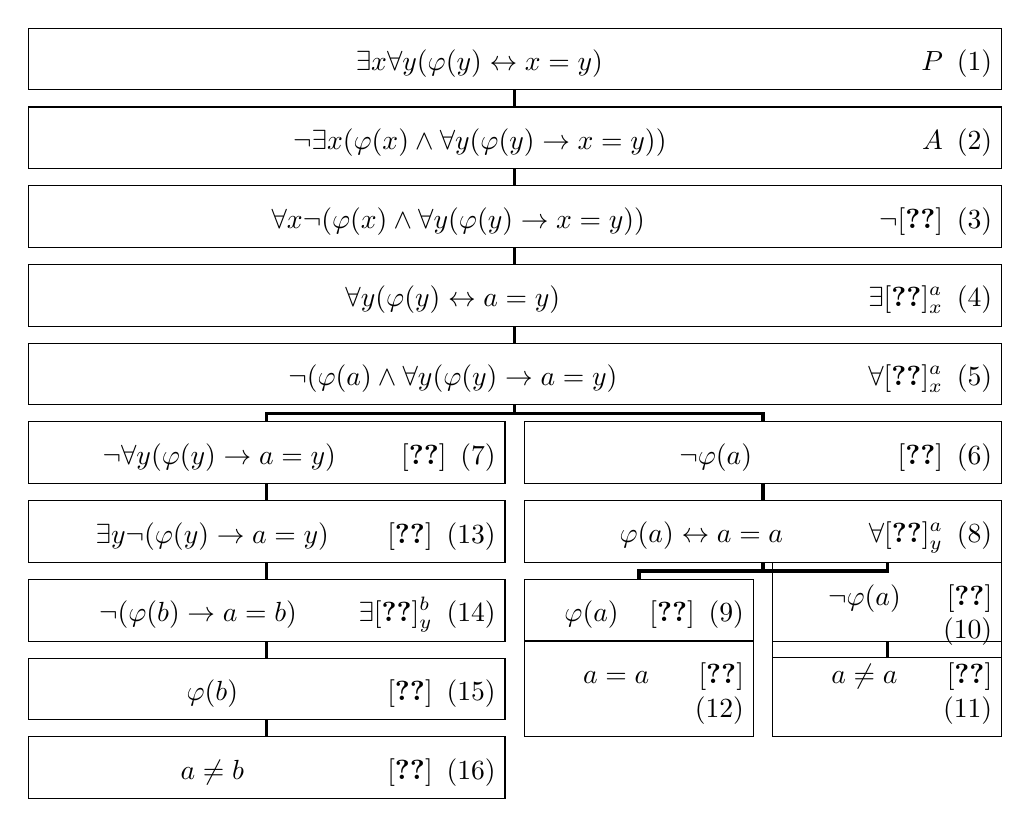
\begin{tikzpicture}
    % These are needed to remove the vertical space around above and below
    % the align and flalign environments
    \setlength{\abovedisplayskip}{0pt}
    \setlength{\belowdisplayskip}{0pt}

    \node[draw, text width=\textwidth] (01) {%
        \begin{minipage}{\textwidth}
            \begin{flalign}
                && \exists x\forall y(\varphi(y)\leftrightarrow x=y) && P
                \label{eq:01}
            \end{flalign}
        \end{minipage}
    };
    
    \node[draw, text width=\textwidth] (02) [below of=01] {
        \begin{minipage}{\textwidth}
            \begin{flalign}
                && \neg\exists x(\varphi(x)\wedge\forall y(\varphi(y)\to x=y)) && A
                \label{eq:02}
            \end{flalign}
        \end{minipage}
    };
    
    \node[draw, text width=\textwidth] (03) [below of=02] {
        \begin{minipage}{\textwidth}
            \begin{flalign}
                && \forall x\neg(\varphi(x)\wedge\forall y(\varphi(y)\to x=y)) && \neg[\ref{eq:02}]
                \label{eq:03}
            \end{flalign}
        \end{minipage}
    };
    
    \node[draw, text width=\textwidth] (04) [below of=03] {
        \begin{minipage}{\textwidth}
            \begin{flalign}
                && \forall y(\varphi(y)\leftrightarrow a=y) && \exists[\ref{eq:01}]^a_x
                \label{eq:04}
            \end{flalign}
        \end{minipage}
    };
    
    \node[draw, text width=\textwidth] (05) [below of=04] {
        \begin{minipage}{\textwidth}
            \begin{flalign}
                && \neg(\varphi(a)\wedge\forall y(\varphi(y)\to a=y) && \forall[\ref{eq:03}]^a_x
                \label{eq:05}
            \end{flalign}
        \end{minipage}
    };
    
    \node[draw, text width=0.48\textwidth] (06) [below of=05, xshift=0.26\textwidth] {
        \begin{minipage}{\textwidth}
            \begin{flalign}
                && \neg\varphi(a) && [\ref{eq:05}]
                \label{eq:06}
            \end{flalign}
        \end{minipage}
    };
    
    \node[draw, text width=0.48\textwidth] (07) [below of=05, xshift=-0.26\textwidth] {
        \begin{minipage}{\textwidth}
            \begin{flalign}
                && \neg\forall y(\varphi(y)\to a=y) && [\ref{eq:05}]
                \label{eq:07}
            \end{flalign}
        \end{minipage}
    };

    \node[draw, text width=0.48\textwidth] (08) [below of=06] {
        \begin{minipage}{\textwidth}
            \begin{flalign}
                && \varphi(a)\leftrightarrow a=a && \forall[\ref{eq:04}]^a_y
                \label{eq:08}
            \end{flalign}
        \end{minipage}
    };

    \node[draw, text width=0.22\textwidth] (09) [below of=08, xshift=-0.13\textwidth] {
        \begin{minipage}{\textwidth}
            \begin{flalign}
                && \varphi(a)&& [\ref{eq:08}]
                \label{eq:09}
            \end{flalign}
        \end{minipage}
    };

    \node[draw, text width=0.22\textwidth] (10) [below of=08, xshift=0.13\textwidth] {
        \begin{minipage}{\textwidth}
            \begin{flalign}
                && \neg\varphi(a)&& [\ref{eq:08}]
                \label{eq:10}
            \end{flalign}
        \end{minipage}
    };

    \node[draw, text width=0.22\textwidth] (11) [below of=10] {
        \begin{minipage}{\textwidth}
            \begin{flalign}
                && a\neq a && [\ref{eq:08}]
                \label{eq:11}
            \end{flalign}
        \end{minipage}
    };

    \node[draw, text width=0.22\textwidth] (12) [below of=09] {
        \begin{minipage}{\textwidth}
            \begin{flalign}
                && a=a && [\ref{eq:08}]
                \label{eq:12}
            \end{flalign}
        \end{minipage}
    };

    \node[draw, text width=0.48\textwidth] (13) [below of=07] {
        \begin{minipage}{\textwidth}
            \begin{flalign}
                && \exists y\neg(\varphi(y)\to a=y) && [\ref{eq:05}]
                \label{eq:13}
            \end{flalign}
        \end{minipage}
    };
    
    \node[draw, text width=0.48\textwidth] (14) [below of=13] {
        \begin{minipage}{\textwidth}
            \begin{flalign}
                && \neg(\varphi(b)\to a=b) && \exists[\ref{eq:13}]^b_y
                \label{eq:14}
            \end{flalign}
        \end{minipage}
    };

    \node[draw, text width=0.48\textwidth] (15) [below of=14] {
        \begin{minipage}{\textwidth}
            \begin{flalign}
                && \varphi(b) && [\ref{eq:14}]
                \label{eq:15}
            \end{flalign}
        \end{minipage}
    };

    \node[draw, text width=0.48\textwidth] (16) [below of=15] {
        \begin{minipage}{\textwidth}
            \begin{flalign}
                && a\neq b && [\ref{eq:14}]
                \label{eq:16}
            \end{flalign}
        \end{minipage}
    };

    \draw[very thick] (01) -- (02) -- (03) -- (04) -- (05);
    \draw[very thick] (05.south) -- ++(0mm, -1mm) -- ++( 0.26\textwidth, 0mm) -- (06.north); 
    \draw[very thick] (05.south) -- ++(0mm, -1mm) -- ++(-0.26\textwidth, 0mm) -- (07.north); 
    \draw[very thick] (06) -- (08);
    \draw[very thick] (08.south) -- ++(0mm, -1mm) -- ++( 0.13\textwidth, 0mm) -- (10.north); 
    \draw[very thick] (08.south) -- ++(0mm, -1mm) -- ++(-0.13\textwidth, 0mm) -- (09.north); 
    \draw[very thick] (09) -- (12);
    \draw[very thick] (10) -- (11);
    \draw[very thick] (07) -- (13) -- (14) -- (15) -- (16);
\end{tikzpicture}
\end{document}
